\documentclass[11pt]{article}
\input{/Users/markwang/.preamble}
\begin{document}


% arg1=pdfurl arg2=pagenum arg3=sectiontitle
\newcommand{\linksection}[3][../../bishop_pattern_recognition_and_machine_learning.pdf]{
    \subsection*{\href[page=#2]{#1}{#3}}
}

\newcommand{\linkinline}[3][../../bishop_pattern_recognition_and_machine_learning.pdf]{
    \noindent\href[page=#2]{#1}{#3}
}

\renewcommand{\norm}[1]{\left\lVert#1\right\rVert}
\renewcommand{\E}[2][]{\mathbb{E}_{#1}\left\{#2\right\}}
\newcommand{\var}[1]{var\{#1\}}
\newcommand{\cov}[1]{cov\{#1\}}
\newcommand{\normal}[1]{\mathcal{N}\left(#1\right)}
\newcommand{\exponents}[1]{exp\left\{#1\right\}}

\newcommand{\bmu}{\boldsymbol{\mu}}

\newcommand{\calR}{\mathcal{R}}
\newcommand{\calC}{\mathcal{C}}
\newcommand{\calD}{\mathcal{D}}


\newcommand{\lebpar}[2]{\frac{\partial #1}{\partial #2}}

\linksection{664}{Appendix C. Matrix Derivatives}


\linksection{155}{Chapter 3 Linear Models for Regression}


\begin{defn*}
    \textbf{Introduction} 
    \begin{enumerate}
        \item \textbf{Problem} Given training set $\{x_n\}$, where $n=1,\cdots, N$ and corresponding target values $\{t_n\}$, the goal is to predict value of $t$ for a new value of $\matr{x}$. 
        \item \textbf{Approach} Construct a function $y(\matr{x})$ whose value is the prediction for some $\matr{x}$. More generally, we aim to model the predictive distribution $p(t|\matr{x})$ as it represent uncertainty of $t$ given $\matr{x}$. We want to find a $y(\matr{x})$ in such a way so as to minimize the expected loss of a chosen loss function (i.e. for squared loss, $y(\matr{x}) = \E[t]{t|\matr{x}}$, the mean of predictive distribution)
    \end{enumerate}
\end{defn*}




\linksection{156}{3.1 Linear Basis Function Models}


\begin{defn*}
    \textbf{Linear Basis Function}
    \begin{enumerate}
        \item \textbf{Model} A linear model with respect to parameters $w_0, \cdots, w_D$ 
        \[
            y(\matr{x,w}) = \sum_{j=0}^{M-1} w_j \phi(\matr{x}) = \matr{w^T \phi(\matr{x})}
            \quad \quad \quad 
            \phi_0(\matr{x}) = 1
        \]
        where $\phi_j(\matr{x})$ are basis functions and $M$ is the total number of parameters in the model, including bias. $\matr{w} = (w_0,\cdots,w_{M-1})^T$ and $\matr{\phi} = (\phi_0,\cdots,\phi_{M-1})^T$. Here is some basis functions 
        \[
            \phi_j(x) = x^j \text{ (polynomial)}
            \quad \quad 
            \phi_j(x) = \exp{-\frac{(x-\mu_j)^2}{2s^2}}  \text{ (gaussian)}
        \]
        \[
            \phi_j(x) = \sigma(\frac{x-\mu_j}{s}) 
            \quad 
            \sigma(x) = \frac{1}{1+e^{-x}} \text{ (logistic)}   
        \]
    \end{enumerate}
\end{defn*}


\begin{defn*}
    \textbf{Maximum Likelihood and Least Squares} Here we show that fitting a linear basis function by minimizing a sum-of-square error function can be motivated as the maximum likelihood solution under an assumed Gaussian noise model. Let target variable determined by $y(\matr{w,x})$ with Gaussian noise
    \[
        t =  y(\matr{x,w}) + \epsilon
    \]
    We can model the predictive distribution with 
    \[
        p(t|\matr{x,w},\beta) = \normal{t|y(\matr{x,w}), \beta^{-1}}
    \]
    For squared loss, the optimal prediction for new value of $\matr{x}$ is given by conditional mean of target variable, 
    \[
        \E{t|\matr{x}} = \int tp(t|\matr{x})dt = y(\matr{x,w})
        \quad \text{i.e. } \E{p(t|\matr{x,w},\beta)} = y(\matr{x,w})
    \]
    Let $\matr{X = \{x_1,\cdots,x_N\}}$ with target $\matr{t} = \matr{\{t_1,\cdots,t_N\}}$, we get likelihood fucntion 
    \[
        p(\matr{t|X,w},\beta) = \prod_{n=1}^N \normal{t_n | \matr{w}^T \matr{\boldsymbol{\phi}(x_n)}, \beta^{-1}}
    \]
    Now we try to minimize likelihood 
    \[
        \ln{p(\matr{t|w},\beta)} 
        = \sum_n \ln{\normal{t_n | \matr{w}^T \matr{\phi(x_n)}, \beta^{-1}}}
        = \frac{N}{2} \ln{\beta} - \frac{N}{2} \ln{2\pi} - \beta E_D(\matr{w})
    \]
    where sum of squared error function is defined by 
    \[
        E_D(\matr{w}) = \frac{1}{2} \sum_{n=1}^N (t_n - \matr{w^T\boldsymbol{\phi}(x_n)})^2
    \]
    Now we find maximum likelihood estimator for $\matr{w}$ and $\beta$,
    \[
        \lebpar{}{\matr{w}} = \sum_{n=1}^N (t_n - \matr{w^T}\boldsymbol{\phi}(\matr{x}_n)) \boldsymbol{\phi}(\matr{x}_n)^T
        \quad \quad \rightarrow \quad \quad 
        \sum_{n=1}^N t_n \matr{\boldsymbol{\phi}(x_n)^T} = \matr{w}^T 
        \left( \sum_{n=1}^N \boldsymbol{\phi}(\matr{x}_n) \boldsymbol{\phi}(\matr{x}_n)^T\right)
    \]
    \[
        \matr{w}_{mle} = \matr{(\Phi^T\Phi)^{-1} \Phi^T t}    
    \]
    where $\matr{\Phi}$ is called the design matrix
    \[
        \matr{\Phi} = 
        \begin{pmatrix}
            \phi_0 (\matr{x}_1) & \phi_1 (\matr{x}_1) & \cdots & \phi_{M-1} (\matr{x}_1) \\
            \phi_0 (\matr{x}_2) & \phi_1 (\matr{x}_2) & \cdots & \phi_{M-1} (\matr{x}_2) \\
            \vdots & \vdots & \ddots & \vdots \\
            \phi_0 (\matr{x}_N) & \phi_1 (\matr{x}_N) & \cdots & \phi_{M-1} (\matr{x}_N) \\
        \end{pmatrix}    
    \]
\end{defn*}

\linksection{161}{3.13 Sequential Learning}


\begin{defn*}
    \textbf{Sequential/On-line Learning} Instead of processing the entire training set in one go, sequential algorithms consider each data points one at a time. \textbf{Stochastic gradient descent} is an online algorithm. Given error function as a sum over errors of all training samples, i.e. $E = \textstyle\sum_n E_n$, $w$ is updated according to 
    \[
        \matr{w}^{(\tau + 1)} = \matr{w}^{(\tau)} - \eta \nabla E_n
    \]
    where $\tau$ is iteration number and $\eta$ is a learning rate parameter. For sum-of-squares error function, this gives 
    \[
        \matr{w}^{(\tau + 1)} = \matr{w}^{(\tau)} - \eta (t_n - \matr{w}^{(\tau)T} \boldsymbol{\phi}_n)\boldsymbol{\phi}_n
        \quad \quad 
        \boldsymbol{\phi}_n = \boldsymbol{\phi}(\matr{x}_n)
    \]
\end{defn*}


\begin{defn*}
    \textbf{Regularized Least Squares} Adding regularization term to an error function to control over-fitting, 
    \[
        E_D(\matr{w}) + \lambda E_W(\matr{w})
    \]
    In case of sum-of-squares error with sum-of-squares regularizer 
    \[
        \frac{1}{2}\sum_{n=1}^N (t_n - \matr{w}^T \boldsymbol{\phi}(\matr{x}_n))^2 + \frac{\lambda}{2} \matr{w}^T \matr{w}
    \]
    The particular choice is called \textbf{weight decay}, an example of parameter shrinkage method because it shrinks parameter to 0. In this case, maximum likelihood estimator has closed form 
    \[
        \matr{w} = (\lambda \matr{I} + \matr{\Phi^T \Phi})^{-1}\matr{\Phi}^T \matr{t}
    \]
    A more general regularizer has form 
    \[
        \frac{1}{2}\sum_{n=1}^N (t_n - \matr{w}^T \boldsymbol{\phi}(\matr{x}_n))^2 + \frac{\lambda}{2} \sum_{j=1}^M |w_j|^q
    \]
\end{defn*}


\linksection{165}{3.2 The Bias-Variance Decomposition}
\linksection{165}{1.1.5 Background on Decision Theory}


\begin{defn*}
    \textbf{Bias-Variance Decomposition} Decision theory for regression consists of choosing a particular estimate $y(\matr{x})$ of value of $t$ for each input $\matr{x}$ such that the expected loss is minimized. For squared loss function, the optimal prediction $y(\matr{x})$ is given by 
    \[
        h(\matr{x}) = \E{t|\matr{x}} = \int t p(t|\matr{x}) dt    
    \]
    We can rewrite the expected loss as 
    \[
        \E{L} = \int (y(\matr{x}) - h(\matr{x})) d\matr{x} + 
        \int (h(\matr{x}) - t)^2 p(\matr{x}) d\matr{x}
    \]
    where the first term is minimized if $y(\matr{x}) = \E{t|\matr{x}}$ and the second term, independent of $y(\matr{x})$ is the variance of the distribution of $t$ averaged over $\matr{x}$, representing the intrinsic variability of the data. We can decompose expectedf loss in terms of bias, variance, and noise 
    \[
        \E{L} = \int (\E[\calD]{y(\matr{x}; \calD)} - h(\matr{x}))^2 p(\matr{x}) d\matr{x} + \int \E[\calD]{y(\matr{x}{\calD}) - \E[\calD]{y(\matr{x}; \calD])}^2} p(\matr{x}) d\matr{x} + \int (h(\matr{x}) - t)^2 p(\matr{x}, t) d\matr{x} dt
    \]
    given a particular dataset $\calD$. The first term is \textbf{squared bias}, represents extend to which average prediction over all data sets differs from the desired regression function. The second term, called \textbf{variance}, measures the extend to which solutions for individual datasets vary around their average (average of $y(\matr{x};\calD)$s), hence measures the extent to which $y(\matr{x};\calD)$ is sensitive to a particular choice of dataset. \\
    As an example, assuming we sample $L$ datasets and fit a model by minimizing regularized squared error function to give $L$ prediction function $y^{(l)}(x)$. The average prediction is estimated by
    \[
        \bar{y}(x) = \frac{1}{L} \sum_{l=1}^L y^{(l)}(x)
    \]
    and the integrated squared bias and integrated variance is approximated by finite sums 
    \begin{align*}
        (bias)^2 \quad &= \quad \frac{1}{N} \sum_{n=1}^N (\bar{y}(x_n) - h(x_n))^2 \\
        variance \quad &= \quad \frac{1}{N} \sum_{n=1}^N \frac{1}{L} \sum_{l=1}^L (y^{(l)}(x_n) - \bar{y}(x_n))^2
    \end{align*}
    Note values of these terms depend on choice of regularization parameter, changes to $\lambda$ adjusts for the bias-variance tradeoff. 
    \begin{center}
        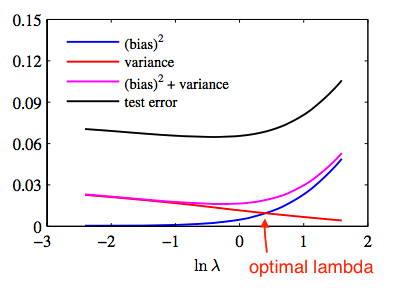
\includegraphics[width=8cm]{regularization_bias_variance_tradeoff.jpg}
    \end{center}
\end{defn*}



\begin{defn*}
    \textbf{Convex Function} A function $f$ is convex if and only if for all $\theta_1,\beta_2$, and for all $\alpha \in [0,1]$, we have 
    \[
        f(\alpha\theta_1 + (1-\alpha)\theta_2) \leq \alpha f(\theta_1) + (1-\alpha)f(\theta_2)    
    \]
\end{defn*}


\begin{defn*}
    \textbf{Newton's Method} is a method for finding successively better approximations to the roots of a real-valued function. The algorithm starts with a function $f$, the derivative $f'$ and the initial guess $x_0$ for the root of $f$, a better approximation is given by updating $x_n$ until convergence
    \[
        x_{n+1} = x_n - \frac{f(x_n)}{f'(x_n)}    
    \]
    $(x_n,0)$ is the intersection of x-axis and the tangent of the graph of $f$ at $(x_n,f(x_n))$. Note the equation of tangen line is given by 
    \[
        y = f'(x_n)(x-x_n) + f(x_n)    
        \quad \quad \rightarrow \quad \quad 
        0 = f'(x_n)(x_{n+1}-x_n) + f(x_n)
    \]
    We can use Newton's Method to find a miminum or maximum of a function $f$ by applying Newton's method to the derivative 
    \[
        x_{n+1} = x_n - \frac{f'(x_n)}{f''(x_n)}
    \]
    In the multivariate case, we have 
    \[
        y = f(\matr{x + \triangle x}) \approx 
        f(\matr{x}) + \nabla f(\matr{x})^T \triangle \matr{x}
        + \frac{1}{2} \triangle \matr{x}^T \matr{H(x)} \triangle \matr{x}
    \]
    Take the gradient
    \[
        \nabla_{\triangle \matr{x}} f(\matr{x} + \triangle \matr{x}) \approx \nabla f(\matr{x}) + \matr{H}\triangle \matr{x}    
    \]
    Setting gradient to zero provides the Newton step 
    \[
        \triangle \matr{x} = -H^{-1} y(\matr{x})
        \quad \quad \rightarrow \quad \quad 
        \matr{x}_{n+1} = \matr{x}_n + \triangle \matr{x}
    \]
    Computing and storing hessian matrix takes $\Theta(n^2)$ memory, infeasible for high dimensional functions. 
    \begin{enumerate}
        \item \textbf{Quasi-Newton Method} Replaces the exact Hessian with an approximation. 
    \end{enumerate}
\end{defn*}

\begin{defn*}
    \textbf{Stochastic Gradient Descent} is a stochastic approximation of the greadient descent optimization and iterative method for minimizing an objective function that is written as a sum of differentiable functions. Sum-minimization problems arise in least squares and in maximum likelihood estimation 
    \[
        Q(w) = \frac{1}{n} \sum_{i=1}^N Q_i(w)    
    \]
    where we want to estimate $w$ such that $Q(w)$ is minimized. A batch gradient descent updates weight with 
    \[
        w = w - \eta \nabla Q(w) = w - \frac{\eta}{N} \sum_{i=1}^N \nabla Q_i(w)    
    \]
    Ther idea is that the summand functions have a simple form that enables inexpensive evalaution of sum and gradient operations for objective function with a good form. In stochastic gradient descent, the gradient $Q(w)$ is approximated by a gradient at a single example 
    \[
        w = w - \eta \nabla Q_i(w)    
    \]
    which perfoms update for each training example, in multiple epochs, such that the algorithm converges. To choose an appropriate setp size by picking a sequence of $\eta_t$ such that 
    \[
        \sum_t \eta_t = \infty 
        \quad \quad \quad \quad 
        \sum_t \eta_t < \infty    
    \]
    satisfied by $\eta_T \propto 1/t$
\end{defn*}


\linksection{171}{3.3 Bayesian Linear Regression}

\linkinline{159}{definition of $p(\matr{t}|\matr{w})$ as product of independent gaussians with $\matr{w}^T \phi(\matr{x}_n)$ as mean}

\linkinline{111}{Formula for marginal and Conditional Gaussian in determining Gaussian posterior}

\begin{defn*}
    \textbf{Parameter Distribution} Bayesian treatment of linear regression, Given a zero-mean isotropic ($\matr{\Sigma}=\sigma\matr{I}$) Gaussian prior and likelihood
    \[
        p(\matr{w}|\alpha) = \normal{\matr{w}| \matr{0}, \alpha^{-1}\matr{I}}
        \quad \quad \quad 
        p(\matr{t}|\matr{w}) = \prod_{n=1}^N \normal{t_n | \matr{w}^T \boldsymbol{\phi}(\matr{x}_n), \beta^{-1}}
    \]
    then we have posterior
    \[
        p(\matr{w}|\matr{t}) = \normal{\matr{w}|\matr{m}_N, \matr{S}_N}
        \quad \quad \quad 
        \matr{m}_N = \beta \matr{S}_N \matr{\Phi}^T \matr{t} 
        \quad 
        \matr{S}_N^{-1} = \alpha\matr{I} + \beta \matr{\Phi}^T\matr{\Phi}
    \]
    Maximization of posterior distribution of log likelihood with respecct to $\matr{w}$ is equivalent to minimization of sum-of-squares error function with the addition of a quadratic regularization term with $\lambda = \alpha/\beta$ 
    \[
        \ln{p(\matr{w}|\matr{t})} = -\frac{\beta}{2} \sum_{n=1}^N \left(t_n - \matr{w}^T \boldsymbol{\Phi}(\matr{x}_n)\right)^2 + \frac{\alpha}{2} \matr{w}^T \matr{w}
    \]
\end{defn*}


\linksection{174}{3.3.2 Predictive Distribution} 


\begin{defn*}
    \textbf{Posterior Predictive Distribution} \href{https://en.wikipedia.org/wiki/Posterior_predictive_distribution}{wiki} Posterior predictive distribution in gaussian linear model is given by marginalizing distribution of prediction $t$ over parameters $\matr{w}$ over posterior distribution of estimated parameters given training dataset $\matr{w}, \matr{t}$.
    \[
        p(t|\matr{t}, \alpha,\beta) = \
        p(t|\matr{w},\beta) p(\matr{w}|\matr{t}, \alpha, \beta) d\matr{w}
    \]
    where integrands refer to \linkinline{158}{3.8} and \linkinline{171}{3.49}. Note the posterior predictive distribution is also a gaussian distribution.
\end{defn*}

\linksection{179}{3.4 Bayesian Model Comparison}


\linksection{179}{3.6 Limitations of Fixed Basis Functions}





\end{document}
